%%==================================================
%% diss.tex for SJTU Master Thesis
%% based on CASthesis
%% modified by wei.jianwen@gmail.com
%% version: 0.3a
%% Encoding: UTF-8
%% last update: Dec 5th, 2010
%%==================================================

% 字号选项: c5size 五号(默认) cs4size 小四
% 双面打印(注意字号设置)
\documentclass[cs4size, a4paper, twoside]{sjtuthesis} 
% 单面打印(注意字号设置)
% \documentclass[cs4size, a4paper, oneside, openany]{sjtuthesis} 


% \usepackage[sectionbib]{chapterbib}%每章都用参考文献
\usepackage{times}
 \usepackage{epsfig}
 \usepackage{graphicx}
 \usepackage{amsmath}
 \usepackage{amssymb}
 \usepackage[lined,boxed,commentsnumbered, ruled]{algorithm2e}
 \usepackage{bm}
 \usepackage{multirow}
 \usepackage{pgfplots}
 %\pgfplotsset{compat=1.9}
 \usepackage{pgfplotstable}

\pgfplotstableset{fixed zerofill,precision=3}
 \usepackage{tikz}
\usetikzlibrary{patterns} %很重要,这个你用everything查下看看是否有这个**code.tex
 \usepgfplotslibrary{groupplots} % 很重要,这个你用everything查下看看是否有这个**code.tex
 \usepgfplotslibrary{patchplots}  % 很重要,这个你用everything查下看看是否有这个**code.tex
 \usepackage{times}
 \usepackage{booktabs}
 \usepackage{array}
 \usepackage{colortbl}
 \usepackage{filecontents}


\newboolean{DOIT}
\setboolean{DOIT}{false}%编译某些只想自己看的内容,编译true,否则false

\newcommand{\todo}[1]{{\textbf{(TODO: #1)}}}
\newcommand{\code}[1]{{\tt#1}}
\newcommand{\refsec}[1]{~\ref{sec:#1}小节}
\newcommand{\reffig}[1]{图~\ref{fig:#1}}

\long\def\comment#1{}

\long\def\myfig#1#2#3#4#5{
\begin{figure}[htb]
  \centerline{\includegraphics[width=#2]{figures/#1}}
  \bicaption[fig:#4]{图索引}{#3}{Fig}{#5}
\end{figure}
}

\long\def\myfigg#1#2#3#4{
\begin{figure*}[!tb]
  \centerline{\includegraphics[width=#2]{figures/#1}}
  \caption{#3}
  \label{fig:#4}
\end{figure*}
}

\definecolor{listinggray}{gray}{0.9}
\definecolor{lbcolor}{rgb}{0.9,0.9,0.9}
\lstset{
  columns=flexible,
  breaklines=true,
  breakatwhitespace=true
  backgroundcolor=\color{lbcolor},
  language=C++,
  captionpos=b,
  tabsize=2,
  %frame=lines,
  frame=shadowbox,
%  numbers=left,
%  numberstyle=\tiny,
%  numbersep=5pt,
  breaklines=true,
  showstringspaces=false,
  basicstyle=\footnotesize,
%  identifierstyle=\color{magenta},
  keywordstyle=\color[rgb]{0,0,1},
%  commentstyle=\color{green},
commentstyle=\itshape\color{black},
  stringstyle=\color{red}
}


%% 行距缩放因子(x倍字号)
\renewcommand{\baselinestretch}{1.3}

% 设置图形文件的搜索路径
\graphicspath{{figure/}{figures/}{logo/}{logos/}{graph/}{graphs}}

%%========================================
%% 在sjtuthesis.cls中定义的有用命令
%%========================================
% \cndash 中文破折号
% 数学常量
% \me 对数常数e
% \mi 虚数单位i
% \mj 虚数单位j
% \dif 直立的微分算符d为直立体。
% 可伸长的数学箭头、等号
% \myRightarrow{}{}
% \myLeftarrow{}{}
% \myBioarrow{}{}
% \myLongEqual{}{}
% 参考文献
% \upcite{} 上标引用
%%========================================


\begin{document}

%%%%%%%%%%%%%%%%%%%%%%%%%%%%%% 
%% 封面
%%%%%%%%%%%%%%%%%%%%%%%%%%%%%% 

% 中文封面内容(关注内容而不是形式)
\title{云搜索正确性快速验证系统的设计与实现}
\author{王根国}
\advisor{赵建军}
\degree{硕士}
\defenddate{2015年1月15日}
\school{上海交通大学}
\institute{软件学院}
\studentnumber{1120379047}
\major{软件工程}

% 英文封面内容(关注内容而不是表现形式)
\englishtitle{Design and Implementation of Fast Proof Generation for Verifying Cloud Search}
\englishauthor{\textsc{Genguo Wang}}
\englishadvisor{\textsc{Jianjun Zhao}}
\englishschool{Shanghai Jiao Tong University}
\englishinstitute{\textsc{School of Software} \\
  \textsc{Shanghai Jiao Tong University} \\
  \textsc{Shanghai, P.R.China}}
\englishdegree{Master}
\englishmajor{Software Engineering}
\englishdate{Jan. 15th, 2015}

% 封面
\maketitle

% 英文封面
\makeenglishtitle

% 论文原创性声明和使用授权
\makeDeclareOriginal
\makeDeclareAuthorization

%%%%%%%%%%%%%%%%%%%%%%%%%%%%%% 
%% 前言
%%%%%%%%%%%%%%%%%%%%%%%%%%%%%% 
\frontmatter

% 摘要
%%==================================================
%% abstract.tex for SJTU Master Thesis
%% based on CASthesis
%% modified by wei.jianwen@gmail.com
%% version: 0.3a
%% Encoding: UTF-8
%% last update: Dec 5th, 2010
%%==================================================

\begin{abstract}
随着计算机硬件和网络带宽的发展,云计算在个人的日常使用中以及商业用途中扮演起了越来越重要的角色。
得益于云存储的大容量,高可靠性,易访问性的特点,越来越多的个人和企业选择了把他们的文档存储到了云存储上。
在对云文档的操作里面,搜索是一项非常常用也非常有用的功能。
怎么保证云搜索的结果是正确的这个问题也变得重要起来。
在这个问题上已经有不少的相关工作,但是一个高效的高扩展性的系统到现在也没有推广开来。

我们在参照了一些已有的验证系统,进行了一些改进,
设计并实现了一个云搜索正确性的快速验证系统。
在该系统中,我们设计的一种树状证明结构来提升证明的生成速度,
并实现了一套轻量级的并行计算框架来用于证明生成的并行计算。
我们的系统有着高效,高扩展性,易维护性的特点。
我们使用了两个测试数据集进行了测试,
测试结果表明我们的系统相比较于原来的计算方法有着平均2倍左右的效率提升,
对于那些本来处理比较慢的情况,比如原来要10s左右的查询,
我们的系统可以达到4倍左右的提升。
我们的系统可以利用多台机器来处理更大规模的数据集,
在我们的实验环境下已经能处理的100GB级别的数据集。
同时,考虑到一些时间效率优先的场景,
我们还设计的一种基于采样的概率验证方式。
该方式提供一种在正确性保证和效率之前的权衡。
	
  	\keywords{\large 云计算 \quad 验证计算 \quad 文档搜索}
\end{abstract}

\begin{englishabstract}

	Nowadays cloud computing is popular in business and daily usage. 
	More and more documents are kept in cloud storage for large storage capicity, high availability and accessible. 
	To providing better service, searching documents on cloud is provided by cloud providers.
	How to proof the correctness of the searching result is an problem coming with this feature.
	Previous work has proposed many useful theories on verifiable computing, such as probabilistically checkable proofs, authHashtable, but an efficient and scalable system is rare.

	We design and implement a fast proof generating system for verifying cloud search based on RSA accumulators, nonmembership witnesses. The system is system and scalable. Evaluation on real datasets shows that our system can speed up the proof generating compared to the raw method and our system can handle datasets with size up to 100GB.

	\englishkeywords{\large Cloud Computing, Verifiable Computing, Document Search}
\end{englishabstract}


% 目录
\tableofcontents
% 插图索引
%\listoffigures
%\addcontentsline{toc}{chapter}{\listfigurename} %将图索引加入全文目录
% 表格索引
%\listoftables
%\addcontentsline{toc}{chapter}{\listtablename}  %将表格索引加入全文目录

% 主要符号、缩略词对照表
%\include{body/symbol}

%%%%%%%%%%%%%%%%%%%%%%%%%%%%%% 
%% 正文
%%%%%%%%%%%%%%%%%%%%%%%%%%%%%% 
\mainmatter


%% 各章正文内容
\chapter{绪论}
\label{chap:introduction}

本章介绍了本课题的研究背景和研究意义。并简单的阐述了本课题使用的研究方法。

\section{研究背景和意义}
随着计算机硬件和网络的不断发展,计算机的使用方式也慢慢的发生了变化,之前的单机使用习惯已经越来越淡化,而对于网络则变得越来越依赖。人们从网络上获取最新的信息咨询,与他人随时随地交流,快速便捷地购物。随着网络的服务的百花齐放,新的计算方式云计算也随之蓬勃发展。

云计算\cite{CloudComputing}是通过网络进行相关服务的部署,使得用户可以远程的在线访问这些服务,例如数据存储,弹性计算。云计算提供商通常使用计算机集群来提供这些服务,并通过虚拟化的方式进行多个用户间资源的共享。与租用硬件不同,云计算按照资源的使用进行计价,这样用户无需担心自己计算需求的变化导致浪费硬件资源,而云服务商通过资源共享,可以最大化的榨取硬件资源的利用价值。云计算使得计算能力变得像电,燃气一样可以流通,用户只需按需购买。

云计算有着大规模、虚拟化、高可靠性、通用性、高扩展性、廉价的特点。得益于这些特点,越来越多的个人和企业选择把数据存放到的云存储上,把自己的业务部署到云计算上。目前各大厂商比如亚马逊,微软,谷歌,阿里云都给用户提供了云计算服务。

云计算其中一种的服务方式是给用户提供数据的存储服务。用户可以把自己的数据放到云平台上,然后只要能在能够访问互联网的环境下,用户就可以随时随地使用任意设备访问自己的数据,方便的进行读写,同步,更新等操作。出了读写这些操作,能够对云存储服务上的数据进行搜索也是用户急切需要的功能。

但和本地环境不同,云计算有着潜在的危险性\cite{CloudComputing}。在享受云计算带来的便利时,我们怎么保证我们得到的是我们真正想要的。比如对于云上的搜索任务,我们怎么保证它真的是按照我们的要求完成任务的呢?目前各大厂商都没有提供一种可以让用户进行验证的机制。云搜索可能会由于服务商的硬件错误,算法错误,或者是受到黑客攻击导致搜索结果是错误的。而没有验证机制,用户可能在毫无察觉的情况下使用了错误的搜索结果而蒙受损失。而且云搜索需要耗费服务商的大量计算资源,服务商为了节省资源可能恶意的只进行部分计算,只返回不完整的结果给用户。这让用户的利益更加无法得到保障。

这些风险的存在,导致很多对安全性正确性比较在意的用户只能放弃了云存储,使得他们无法享用云计算带来的那些好处。而服务商也因此失去了不少用户资源。
针对这些情况,如果能找到一种低成本的验证方式,那么就可以很好的解决了这个问题。设想有一种方式,服务商付出完全可以承受额外计算和存储压力就可以为每一次搜索计算一个证明返回给用户,同时用户也可以快速有效地进行正确性验算,不至于影响到用户体验。这对于云计算服务商以及用户都是非常有意义的。

\section{国内外研究现状}
本节我们介绍下关于文档搜索与结果验证方面的国内外研究现状。

\subsection{文档搜索方法和结果验证的关系}
		云存储上的文档搜索和本地的文档搜索没有什么本质的区别。这一块已经积累了很多研究以及有很多成熟的产品。对于不同的搜索方法,验证结果的正确的方法也有很大的差异。所以我们打算只选择一种最普遍的全文搜索的方法来进行我们的研究:先对文档进行预处理,然后建立反向索引。通过反向索引进行多关键词的搜索。
\subsection{搜索结果验证}
				 验证或者保证第三方计算的正确性,并不是一个新的方向。在早期,交互式证明系统就被提出来用于证明第三方计算的正确性。交互式证明系统分为一个假设计算力无限的证明者和计算力有限的验证者。通过类似提问回答的交互方式,证明者试图证明它给出的结论是正确的,而验证者则要判断证明者的结论是否是可信的。Arthur–Merlin协议实现了一种概率上宽容了的交互性验证系统。还有一类是概率验证模型,它通过随机的检测一些部分的结论,来一定概率上确定该结论是否是正确的。最近的在这两类上一些研究在时间空间复杂度上有着极大的提高。但是生成证明还是比计算出结果要耗费上一个数量级以上的时间,这极大的影响了它们的可用性。除了验证计算结果这一方式外,也有研究提供一些计算结果保证正确的机制。比如在执行前验证可执行文件的完整性,提供第三方监控层监控执行过程。但这无法保证云计算提供商或者破坏分子不去攻击内存中的数据,或者更改执行结果。具体到验证云计算搜索结果正确性验证,有研究提供了一种使用不可逆哈希强迫云计算提供商要进行正确的搜索计算才能给出哈希验算结果。该方法有不错的时间效率,但是也有很多局限性,比如不能支持单个搜索。
\subsection{数据安全}
						云存储依赖于第三方,难免会涉及敏感数据,数据安全是云计算研究中的关键问题。有研究在不安全存储上建立安全文件系统。为了保证数据的隐私性,可以采用对称加密方法(比如,AES)对数据加密之后进行上传,这样就可以保证除了密钥拥有者,别人无法看到数据的明文。

						    涉及到搜索,我们可能要需要把索引文件上传到服务端。为了保证索引的安全性,有研究给出,可以使用对称加密给索引的每个关键词都加密,这样就可以防止信息泄露。对于词频信息,有研究指出可以将不同关键词进行组合来进行伪造隐藏。

\section{研究内容}
本课题分析目前现有的搜索验证方式没有一个高效的可以扩展的系统,提供一个对现有的验证方式进行了效率上的提高,实用性增强的系统。

现有的一些验证方法,多数都只是一些比较抽象的数学和逻辑上的框架,比较缺乏实际可用的系统。少数的代码实现中,基本都是比较直接的计算,没有进行一些系统的设计和一些结构的更改来进行优化。为了实现一个高效的云搜索验证系统,我们主要从事了搜索及验证算法的选择,验证系统的设计,验证系统的优化这几个方面的研究。

\section{论文结构}
本论文主要描述了我们的云搜索正确性快速验证系统的设计与实现,并着重描述其中的整体框架与一些比较重要的细节设计。
余下的部分组织如下。第二章介绍了本课题涉及到的相关工作,主要介绍了RSA Accumulator和一套验证机制。第三章介绍了我们的系统可能的应用场景。第四章描述了我们系统的整体架构以及一些优化方案。第五章我们对本系统做了实验评估,并对实验结果做了简单的分析总结。第六章对本课题进行简要的总结以及对本课题的后续研究做了展望。

\section{本章小结}
本章介绍了我们的课题的研究背景和意义。在目前云计算蓬勃发展的现状下,很多用户选择把数据存储到云服务上,随时随地进行访问查询。由于云计算有潜在的危险性,用户需要的查询结果可能会是错误的,并导致用户利益承受损失。而目前没有一个通用的高效的系统来保证用户搜索结果的正确性。针对这一问题,我们设计并实现了一个较为高效,易于扩展的系统。本章还介绍了对于本课题相关的计算验证方面的目前研究现状。在最后,本章对于本论文的后续章节的内容和结构做了简单的介绍。

\chapter{相关工作}
\label{chap:relatedwork}
在本章,我们介绍本课题用到的一些相关的工作。主要的介绍了我们系统使用的云搜索验证机制。该机制使用了RSA Accumulator\cite{goodrich2002efficient,verifiableindex}来进行集合元素的存在性验证。接下来,我们先介绍RSA Accumulator,然后再介绍下基于RSA Accumulator的验证机制。

\section{RSA Accumulator}
RSA Accumulator是One-way Accumulator\cite{benaloh1994one}的一种直观的扩展。它可以用来计算集合的membership witness(用于证明一个元素属于一个集合)和nonmembership witness(用于证明一个元素不属于一个集合)。
取X = \{$x_1, x_2, ... , x_{|X|}$\}作为输入集合,其中的每个元素$x_i$都是质数。然后我们选择两个比较大(比如说1024位的)的质数。随后我们取与n=pq互质的一个数g作为底数。那么集合X的Accumulator为:
\begin{equation} c = g^{\prod_{i = 1}^{|X|} x_i}\ mod\ n \end{equation}

我们可以把这个Accumulator理解成类似集合的指纹。任何人在不得知p和q的情况下,是无法在多项式时间内找到另一个集合$Y \neq X$,且集合Y的Accumulator也是c。这个性质可以有强RSA假设来推导出。

我们取X的子集$X^{\prime} = \{x_{i_1}, x_{i_2}, ... , x_{i_{|X^\prime}}\}$, 那么$X_\prime \subseteq X$的Membership Witness为:
\begin{equation} \label{eq:w} c_{X^\prime} = g^{\prod_{x \in X - X^\prime} x}\ mod\ n \end{equation}

有了这个Membership Witness, 我们如果要证明$X_\prime \subseteq X$ 只需要验证下式是否成立:
\begin{equation} \label{eq:vw} c_{X^\prime}^{\prod_{x \in X^\prime} x} = c\ mod\ n\end{equation}
从式子\ref{eq:vw}可以看出,对于$X_\prime \subseteq X$的验证,我们所需要关于集合X的信息只要知道它的Accumulator c就行了,而不用知道它包含哪些元素。

我们另去集合 $Y = \{y_1, y_2, ... , y_{|Y|}\}$,它的每个元素$y_i$都是质数,且 $Y \bigcap X = \phi$。那么集合Y相对于X的Nonmembership Witness是这样一个二元组(a, d) 其中
$au + bv = 1, d = g^{-b}\ mod\ n, u = \prod_{x \in X} x, v = \prod_{y \in Y} y$

如果我们要证明 $Y \bigcap X = \phi$,只需要验证下式是否成立:
\begin{equation} \label{eq:vnw} c_a = d^v g\ mod\ n \end{equation}

\section{验证机制}
The verifiable cloud search receive user's query and return the result document set with their rank weight and query proof for verify the query result. Illustrated in \cite{verifiableindex}, the process of verifiable cloud search consisted of three steps: build verifiable index, cloud indexing, verify proof.

Build verifiable index: 
To use the RSA Accumulator, the verifiable index is model as a map from a term $t_i$ to a set of docId tuples, where docID means a document ID which contains term $t_i$ and w is term $t_i$'s weight in this document.

For each term, the client compute the accumulator of the set and keep a local copy.

Cloud Indexing:
When received a query, the cloud server lookup verifiable index and find each query term $t_i$'s index data. Then the cloud server compute the intersection of the index data which is a set of docId of all query terms. The query result consisted of the intersection set of documents IDs and (docId,tuple) for each term and each docId in the intersection.

Let $S_i$ be the set of document IDs for term $t_i$. For a query composed of term $t_i$ and $t_j$, the intersection $S = S_i \bigcap S_j$ contains the document that have both terms.
The proof consisted of a correctness proof and an integrity proof. The correctness is the witness for $S \subseteq S_i$ and $S \subseteq S_j$ and the integrity proof is the nonmembership witness for $(S - S_i) \bigcap S_j = \phi$
With the both correctness proof and integrity proof, we can proof $S = S_i \bigcap S_j$

Verify proof:
The client verify the result returned from the server with proofs. The client verify the correctness proof by checking the witness using equation 3 and verify the integrity proof by checking the nonmembership witness using equations 4.


\chapter{应用场景}
\label{chap:application}
在这篇论文中,我们设计并实现了一个云搜索正确性的快速验证系统,
该系统能够对于搜索结果快速地生成结果证明。云服务商在返回搜索结果的时候会把结果证明也返回给用户。有了这个证明,用户就可以在本地进行搜索结果正确性的验证。相比于原有的一些验证方案,我们的系统有着高扩展性、高效率的特点。这些特点也让我们的系统有了比较不错的应用场景。在本章中,我们讨论下我们的系统的应用场景。

首先我们的系统需要用户在本地对文档创建索引,以及进行一些必要的计算。所以那些直接在云端的生成新的文件的场景就不太合适使用该系统了,比如在线文档编辑系统。
我们系统的主打功能是对云搜索的正确性进行验证,所以最适合的场景肯定是在云服务上的,既有文档搜索需求的,同时也要有正确性保证需求的场景。
综合考虑下,我们认为本系统的应用场景为针对正确性敏感用户,提供文档存储和文档全文关键词搜索的云存储系统。

目前,我们的系统可以主要面向一般的用户文档。对于一般用户的文档,它一般不会像多媒体文件那么拥有巨大的尺寸,这样方便了我们进行快速地建立索引以及进行一些事先的计算。

下面我们举一个具体的应用场景为例。

\section{云档案管理系统}
一般公司和政府的常规的档案管理都是在企业内部搭建一个服务器,然后部署一套档案管理系统软件\upcite{DocumentManage}。在本地部署这样的一套系统有着可以自己定制各种功能、安全性比较高、可以有效避免信息泄露及第三方恶意攻击等诸多优点。但是有些时候,企业或政府部门不需要很复杂的功能,只是需要对于档案的进行增删改查就行。这些功能一般的云服务就可以提供。
而且企业或者政府部门一般有很多报销、税收、政策、审批之类的档案,还有一些档案的扫描件,都是需要大量的存储。这一点云服务也很适合解决。
但是考虑到安全性,比如信息泄露,还有第三方的计算结果正确性无法保证等问题,云服务这种方式就被排除在外了。这个时候,企业或政府部分就只能自己在本地搭建一套档案管理系统。

相比于使用云服务来说,对不是以IT为主要职责企业和政府部门,自己在本地部署一套档案管理系统是需要承受不少额外成本的,而且系统的可靠性和稳定性也无法做到像云服务那么好。


而我们的云搜索正确性快速验证系统可以通过加密来保证档案内容的安全性,可以通过正确性验证来保证用户对档案进行的查询操作的都是正确的。而且我们系统的高效性可以给用户提供友好的体验。我们系统的可扩展性使得它可以容易地应对各种规模的档案数据。

\myfig{app.eps}{4.5in}{云档案管理系统应用场景}{app}{Application for cloud document management}
我们在图\ref{fig:app}描述了将云搜索快速验证系统应用到档案管理的场景。用户在迁移到该系统时,首先要在本地对档案文件建立可验证索引,然后将档案加密再上传到云服务上。之后在日常使用时,用户需要查找某些档案,
那么他只需要向云档案管理系统发送查询请求,然后在云端返回结果和结果证明之后,对结果证明进行验算,就可以保证这次的查询是正确的。

考虑到档案可能不一定都是以文档的形式存在,比如说很多文档的扫描件都是以图片的形式存在的。我们可以通过简单地扩展,使得我们的系统增加对图片这类扫描件的支持。对于一些图片之类的文件,我们可以使用一些文字识别的技术或者直接是人工标注的方法来建立索引,这样我们的系统也能处理这些非文本的数据了。

\section{本章小结}
本章探讨了下我们系统解决的问题和应用场景。针对我们系统可以给云搜索增加搜索结果验证的功能,我们的应用场景主要瞄准那些对数据安全性,对结果正确性有着高要求的场景。按照这类场景的标准,我们以云档案管理系统为例,展示了我们系统的在这种场景下的应用方式。

\chapter{设计}
\label{chap:design}


本章我们将介绍云搜索正确性的快速验证系统的整个系统构造。首先,我们会介绍该系统的整体框架,介绍它是有那些部分组成的,每个部分是什么功能的以及各个部分之间是怎么交互的。然后,我们会介绍整个系统里面一些重要的细节,比如为了提升整体效率而设计的一些方案,比如树状的证明结构。

\section{系统的整体架构}

考虑到高可靠性,扩展性,高可维护性的要求,我们将系统分为了Search Server, Search Client, Query Node, Correctness Server, Integrity Server这几个组成部分。
Search Client:是负责发起搜索任务的模块。该模块接受用户的输入,然后把该搜索关键词发送到Search Server进行查询。在服务端返回结果后,Search Client可以对该结果以及随结果返回的证明进行验证,以此来判断该结果是否正确。
Search Server: 如其名所言,是负责接收搜索任务的模块。该模块接收从Search Client发送过来的搜索请求,对该搜索请求进行一些初步处理,比如去除一些无关词语,然后会把本次搜索的关键词发送到各个Query Node。每一个Query Node会返回他们拥有的和本次搜索结构相关的索引内容。在各个Query Node返回它们的查询结果后,Search Server会对这些结果进行整合,这样就得到了一个完整的搜索结果。然后,Search Server会把这个结果分别发送到Correctness Server和Integrity Server去进行证明的计算。等到证明计算完成,Search Server就把搜索结果和证明一起返回给客户端。到这里,本次搜索的过程就结束了。
Query Node: Query Node负责一部分的索引查询。在我们的系统中,索引被按照尺寸大小分成了M份。如果我们有N个Query Node, 我们用0,1,2…N-1进行编号。编号为i的Query Node负责编号为i, i+N, i+2*N,…的索引文件。当一个查询到来的时候,Query Node查询自己负责的那部分索引里面是否有本次搜索包含的关键词部分,如果有就返回相应的内容,如果没有就告知没有。
Correctness Server: 计算正确性证明。Correctness Server使用了稍后会介绍的树状证明结构。该结构能够将正确性计算从一次非常耗时的计算分解成多个可以快速计算的小任务,以此来充分利用计算机集群以及多个CPU核来加快计算的速度。
Integrity Server: 计算完整性证明。该计算与正确性证明是同时进行的,来加快整个证明的计算速度。
在我们的系统中,每个模块都是单独的进程。模块这件是通过HTTP协议进行通讯,所以各个模块可以随意的部署到不同的机器,这样可以充分利用整个计算机集群,以提供非常不错的可扩展性。
\myfig{framework.eps}{3.5in}{系统的整体框架 }{des:structure}

\section{树状证明}

我们取 D = \{$d_1$\, $d_2$, ..., $d_n$\}表示某个关键词的倒排索引里面的文档集合。
我们取D的子集 S = \{$d_{i_1}$, $d_{i_2}$, ..., $d_{i_m}$\},那么公式提的方法,我们要计算S属于D的Membership Witness的话,我们将近需要对集合D里面的每一个元素进行累乘,然后进行一次乘方计算。
在我们的设计里面使用了GMP这个库进行高精度数学计算。经过测试,我们发现连续乘方的速度比先累乘的速度要快很多。于是我们就采用了连续乘方的方式。但连续乘方这样的计算方式有一个问题,那就是计算步骤是相互依赖的,于是没法使用并行计算进行加快。
文章【】提出了一种RSA树的结构用来进行高效的集合元素的存在性证明。我们在其基础上设计了树状证明这样的结构。
我们取e为大于1的整数,对于文档集合D,我们对其进行树状结构的构建。为了便于描述,我们把这样的树叫做T(e, D),它有如下的特点:
\begin{enumerate}
  \item T(e, D) 是一颗三层的树
  \item 叶子节点保存文档的质数表示。第i叶子节点保存对应文档$d_i$的质数表示。
  \item T(e, D) 有 m = $\lceil \frac{m}{e} \rceil$ 中间层节点。第i个中间层节点 $m_i$ 存储它所有子节点组成集合的Accumulator。
  \item 除了最后一个中间层节点,每个中间层节点有且仅有e个子节点。最后一个中间层节点有不多于e个的子节点。
\end{enumerate}

对于这样的结构,我们如果要证明某个叶子存在,可以先证明它属于某个中间层节点,然后再证明这个中间层节点存在,也就是证明这个中间层节点属于根节点。按照这个思路,我们取M = \{$m_0, m_1, ..., m_{m-1}$\},G($m_i$) = \{$d_j$ | $d_j$ 是 $m_i$的子节点 \}, 取D的子集S = \{$d_{i_1}$, $d_{i_2}$, ..., $d_{i_m}$\}。 那么我们对于 $S \subseteq D$ 是如下这样:
\begin{enumerate}
  \item 把S拆分成 $S_0$, $S_1$, $S_{m-1}$,其中 $S_i$ = $S \bigcap G(m_i)$。 也就是说 $S_i$ 包含S中的那些属于第i个中间层节点的元素。
  \item 对于每个非空的 $S_i$, 我们计算 $S_i \subseteq G(m_i)$的证明: $p_i = g^{\Pi_{\mu \in G(m_i) - S_i} r(\mu)} mod N$, 这里 $r(\mu)$ 是 $\mu$的质数表示。 
  \item 对于每个非空的 $S_i$, 我们计算 $m_i \in M$的证明:$q_i =  g^{\Pi_{\mu \in M, \mu \ne m_i} r(\mu)} mod N$
  \item 我们的树状证明由全部的$(S_i, p_i, q_i, m_i, a)$元组组成 , 这里的a是集合M的Accumulator.
\end{enumerate}

有了这样的树状证明,我们就可以按照以下步骤进行验证:
\begin{enumerate}
  \item 检查 $\cap S_i = S$来证明S中的每个元素都没有遗漏,都包含在了证明中。
  \item 检查 $p_i^{\Pi_{\mu \in S_i} \mu} = m_i mod N$来证明 $S_i \subseteq G(m_i)$
  \item 检查 $q_i^{m_i} = a$ 来证明 $m_i in M$
  \item 检查 a 是否和客户自己计算并保存在本地的一样,一次来保证这个树状结构不是云端随意构造的
\end{enumerate}

使用树状证明的好处是:1. 对于$S_i$是空集的情况,我们是不需要进行计算的。2. 我们在将S划分成$S_0$, $S_1$, $S_{m-1}$之后, 对$S_i$它们进行的计算是没有相互依赖关系的,我们可以使用并行计算来进行加速。

树状证明有着 O(|S|) 的空间复杂度。这个和搜索结构的空间复杂度是一致的。所以树状证明不会使得整体的空间复杂度增加,是完全可以接受的。

\myfig{tree.eps}{3.5in}{由20个文档组成, e = 4的树状结构}{des:tree}
\section{事先计算}
在证明的生成过程中,我们用到了很多计算量很大且重复使用次数很多的一些数据。对于每个文档的质数表示。。。
\section{Worker任务分配机制}
\section{基于概率的验证}
我们的系统在证明生成上的效率相比原来的方法有了不少提升。但对于那些对证明要求不高的使用场景,每次搜索的时候都要去计算证明的话,是比较浪费计算资源,也增加了用户的等待时间,是得不偿失的。

对于那样的场景,我们提出了一种基于概率的验证方式。对于搜索,我们提供两种模式,一种是非验证搜索,该种模式下服务端只需要返回搜索结果,无需进行证明的生成,另一种是验证搜索,该种模式下服务端要同时返回结果以及证明。

假设云服务商的搜索不是完全正确的,假设其错误概率为p。在一般情况下,我们使用非验证搜索这个效率更高,使用资源更少的搜索方式。比如说我们进行了n次非验证搜索。这时由于没有证明,我们是不知道云服务商给的结果是否是正确的。然后我们在这n非验证搜索里面抽取m次进行验证搜索。

为了防止云服务商对于验证搜索时给正确结构,而非验证搜索时给错误的结果,我们首先要比较验证搜索和非验证搜索的结果,如果不一致,说明云服务上的搜索是不正确的。

在验证了两种搜索结果一致后,我们再对m个验证搜索的结果进行验证。由于云服务商的错误概率是p,那么在这m个验证中,我们发现云服务商是有问题的概率是$1-(1-p)^m$

我们在表TODO中列举了一些数据结果,从这些结果来看,我们只需要不多的检测就能有很高的概率来检测出来云服务商是否是有问题的。

%\chapter{实现}
\label{chap:implementation}

在本章我们将介绍云搜索正确性的快速验证系统的整个系统构造。首先,我们会介绍该系统的整体框架,介绍它是由哪些部分组成的,每个部分负责什么功能以及各个部分之间是怎么交互的。
然后,我们会介绍为了解决正确性证明计算速度慢而设计的树状结构证明,以及一种将树状结构证明推广到完整性证明计算的方法。我们还介绍了一个为了方便树状结构证明的并行计算而设计实现的轻量级计算框架。

\section{系统的整体架构}

在第\ref{chap:design}章,我们介绍了基于RSA Accumulator的验证机制。围绕这个验证机制,我们设计实现了云搜索正确性的快速验证系统。按照该验证机制的特点,
我们将系统分为了线下和线上两个部分。线下部分主要负责文档的预处理、生成索引、预先计算质数表示等任务。
线上部分负责的是实时搜索部分。
具体的,考虑到高可靠性、扩展性、高可维护性的要求,我们对系统进行了模块化的设计。
线下部分主要由Index Generator和Prime Manager这两个模块组成。
线上部分比较复杂,主要由Search Client、Search Server、Query Node、Correctness Server、Integrity Server这几个模块组成。我们会在后续的内容中对这些线下线上的模块分别进行介绍。

在我们的系统里,每个模块都是一个可以单独启动的进程,模块之间使用HTTP协议进行交互。采用这样设计的原因主要是:1. 采用单独的进程可以让每个模块进行单独的部署,而不需要都部署到一台机器上,这样使得系统有比较好的可扩展性;2. HTTP协议是一种使用得非常广泛也非常易于使用的协议,采用HTTP协议可以让我们的系统更加容易进行调试也方便了一些扩展模块的开发。

我们的系统采用了C++来进行实现,用到了很多boost库的内容,比如利用了其中的Asio来进行异步的HTTP请求。在高精度计算方面,我们采用了NTL这个C++库\upcite{NTL},并采用了GMP加速。

下面我们按照模块对云搜索正确性的快速验证系统进行介绍。

\myfig{framework.eps}{3.5in}{系统线上部分的整体框架 }{des:structure}{Structure of our system's online part}

\subsection{Index Generator}
Index Generator是一个单独的工具,它不需要和别的模块进行交互。它主要负责的对于一个文本集合进行可验证索引的建立操作。我们采用了Indri Indexer\upcite{Indri}来生成倒排索引。在生成了倒排索引之后,我们从中抽取出我们需要的内容,用来生成可验证索引。对于生成的可验证索引,我们以文件的形式存储到磁盘上。索引的数据比较大,为了减少单个文件的体积,同时也为了方便使用多模块处理,我们将索引数据使用一致性哈希\upcite{ConsistentHash}的方式存储到多个文件中。生成的索引数据文件组织如下:
\begin{itemize}
\item meta.txt 存储索引数据的元信息,包括索引版本、文档总数目、单词总数目、索引文件的数目、平均的文档长度等信息。
\item term\_map.txt 存储单词到单词编号的映射。
\item ch\{0,1,..,M\}.txt M个文件。M由用户指定。存储所有单词编号到(docID, w)二元组集合的映射。我们使用单词的SHA1值作为Key,然后使用一致性哈希将其分配到对应的ch.txt文件。如果各个文件的索引数目不均匀,我们可以采用加大M值的方式来解决。
\end{itemize}

\subsection{Prime Manager}
Prime Manager这个模块的作用是使用事先计算好的质数表示来加快搜索结果的证明的计算。在证明的计算里面,我们需要使用到文档编号、索引数据、单词编号等元素的质数表示。计算质数表示是一项比较费时间的计算,而且在我们的系统中有着非常高的使用频率,且包含很多重复计算的情况。所以,我们采用了事先计算的方式来避免线上系统在计算质数表示上浪费时间。我们对每一个文档编号、每一个单词的索引数据都事前计算好质数表示,存储到文件中。在系统使用时,只需要到Prime Manager查询相应的质数表示,而不再需要进行繁重的计算。

在事先计算质数表示时,对于大的数据集,我们使用MPI开发了一个程序来进行并行计算。在并行计算的任务划分中,由于每个单词的索引数据的大小并不一致,我们没有简单的按照单词进行任务划分,而是按照索引条目进行任务的划分。从系统的运行情况来看,按照索引条目进行划分的策略确实加快了这个计算过程。

\subsection{Search Client}
Search Client是负责发起搜索任务并对搜索结果进行验证的模块。该模块接受用户的输入,然后把该搜索关键词发送到Search Server进行查询。在服务端返回结果后,Search Client可以对该结果以及随结果返回的证明进行验证,以此来判断该结果是否正确。

在我们目前的系统中,Seach Client支持命令行交互的查询方式和一次性从文件中载入批量的查询这两种方式。在后续,会增加更加用户友好的图形交互界面。

\subsection{Search Server}
Search Server: 如其名所言,是负责接收搜索任务的模块。
该模块接收从Search Client发送过来的搜索请求,对该搜索请求进行一些初步处理,
比如去除一些无关词语,然后会把本次搜索的关键词发送到各个Query Node。
每一个Query Node会返回它们拥有的和本次搜索内容相关的索引内容。
在各个Query Node返回它们的查询结果后,Search Server会对这些结果进行整合,
这样就得到了一个完整的搜索结果。然后,Search Server会把这个结果分别发送到Correctness Server和Integrity Server去进行证明的计算。
等到证明计算完成,Search Server就把搜索结果和证明一起返回给客户端。
到这里,本次搜索的过程就结束了。

\subsection{Query Node}
Query Node是负责索引查询的模块。在我们的系统中,索引被按照一致性哈希的方式分成了M份。如果我们有N个Query Node, 我们用0,1,2…N-1进行编号。编号为i的Query Node负责编号为i, i+N, i+2*N,…的索引文件。当一个查询到来的时候,Query Node查询自己负责的那部分索引里面是否有本次搜索包含的关键词部分,如果有就返回相应的内容,如果没有就告知没有。

\subsection{Correctness Server}
Correctness Server是负责计算正确性证明的模块。Correctness Server使用了稍后会介绍的树状证明结构。该结构能够将正确性计算从一次非常耗时的计算分解成多个可以快速计算的小任务,以此来充分利用计算机集群以及多个CPU核来加快计算的速度。

\subsection{Integrity Server}
Integrity Server是负责计算完整性证明的模块。该计算与正确性证明是同时进行的,来加快整个证明的计算速度。目前,我们系统的完整性证明计算就是简单按照验证机制里面介绍的步骤进行的。在本章后面的部分,我们有介绍到一种将树状结构证明应用到完整性证明计算的方法。在后续工作中,我们可以将那个方法实现到本模块中。

\section{树状结构证明}
在我们系统设计的初期,我们只是简单的使用并行计算正确性证明和完整性证明来加速证明的计算。
经过一些测试之后,我们发现这个计算速度还比较慢。对于一些文档集合比较大的搜索结果,生成证明的时间可以高达几十秒。在使用了性能调优工具进行性能瓶颈检测后,我们发现正确性证明的生成占用了大部分的计算时间。在经过一些了调查和尝试之后,我们设计并实现了树状结构证明来加快正确性证明的计算。

\subsection{树状结构证明的设计}

\myfig{tree.eps}{3.5in}{由20个文档组成, e = 4的树状结构}{des:tree}{Tree structure with 20 documents and e = 4}
我们取 D = $\{d_1, d_2, ..., d_n\}$表示某个关键词的倒排索引里面的文档集合。
我们取D的子集 S = $\{d_{i_1}, d_{i_2}, ..., d_{i_s}\}$,那么按照公式\ref{eq:w}提的方法,我们要计算集合S属于集合D的Membership Witness的话,我们需要对集合D里面的每一个元素进行累乘,然后进行一次乘方计算。
在我们的设计里面使用了GMP这个库进行高精度数学计算。经过测试,我们发现连续乘方的速度比先累乘的速度要快很多。比如计算$g^{ab}$,连续乘方指先计算$g^a$,再计算$(g^a)^b$;先累乘指先计算$ab$,然后计算$g^{(ab)}$。于是我们就采用了连续乘方的方式。但连续乘方这样的计算方式有一个问题,那就是计算步骤是相互依赖的,于是没法使用并行计算进行加快。
文章\cite{papamanthou2008authenticated}提出了一种RSA树的结构用来进行高效地集合元素存在性验证。我们在其基础上设计了树状结构证明这个利用树状结构来计算正确性证明的方式。
我们取e为大于1的整数,对于文档集合D,我们对其进行树状结构的构建。为了便于描述,我们把这样的树叫做T(e, D),它有如下的特点:
\begin{enumerate}
  \item T(e, D) 是一颗三层的树
  \item 叶子节点保存文档的质数表示。第i个叶子节点保存文档$d_i$的质数表示。
  \item T(e, D) 有 m = $\lceil \frac{n}{e} \rceil$ 中间层节点。第i个中间层节点 $m_i$ 存储它所有子节点组成集合的Accumulator。
  \item 除了最后一个中间层节点,每个中间层节点有且仅有e个子节点。最后一个中间层节点有不多于e个的子节点。
\end{enumerate}

在图\ref{fig:des:tree}中我们展示了由一个包含20个文档的集合生成的树状结构。
对于这样的结构,我们如果要证明某个叶子存在,可以先证明它属于某个中间层节点,然后再证明这个中间层节点存在,也就是证明这个中间层节点属于根节点。按照这个思路,我们取$M = \{m_0, m_1, ..., m_{m-1}\}$,$G(m_i) = \{d_j$ | $d_j$ 是 $m_i$的子节点 \}, 取D的子集$S = \{d_{i_1}, d_{i_2}, ..., d_{i_s}\}$。 那么我们对于 $S \subseteq D$ 的树状结构证明是按照如下步骤计算的:
\begin{enumerate}
  \item 把S拆分成 $S_0$, $S_1$, $S_{m-1}$,其中 $S_i$ = $S \bigcap G(m_i)$。 也就是说 $S_i$ 包含S中的那些属于第i个中间层节点的元素。
  \item 对于每个非空的 $S_i$,我们计算 $S_i \subseteq G(m_i)$的Membership Witness:$p_i = g^{\Pi_{\mu \in G(m_i) - S_i} r(\mu)}\ mod\ N$,这里 $r(\mu)$ 是 $\mu$的质数表示。 
  \item 对于每个非空的 $S_i$,我们计算 $m_i \in M$的Membership Witness:$q_i =  g^{\Pi_{\mu \in M, \mu \ne m_i} r(\mu)}\ mod\ N$。
  \item 我们的树状证明由全部的$(S_i, p_i, q_i, m_i, a)$元组组成 , 这里的a是集合M的Accumulator。
\end{enumerate}

有了这样的树状结构证明,我们就可以按照以下步骤进行验证:
\begin{enumerate}
  \item 检查 $\cap S_i = S$来证明S中的每个元素都没有遗漏,都包含在了证明中。
  \item 检查 $p_i^{\Pi_{\mu \in S_i} \mu} = m_i\ mod\ N$来证明 $S_i \subseteq G(m_i)$。
  \item 检查 $q_i^{m_i} = a$ 来证明 $m_i \in M$。
  \item 检查 a 是否和客户自己计算并保存在本地的一样,以此来保证这个树状结构不是云端随意构造的。
\end{enumerate}

使用树状证明的好处是:1. 对于$S_i$是空集的情况,我们是不需要进行计算的;2. 我们在将S划分成$S_0$, $S_1$, $S_{m-1}$之后,对$S_i$这些小集合进行的计算之间是没有相互依赖关系的,我们可以使用并行计算来加速这个计算过程。而且,中间层节点属于根节点的证明$q_i$可以事先计算。这样,在整个计算过程中,我们需要计算的只有$p_i$。
在我们的系统中,我们设计了一个叫Worker任务分配机制的计算框架来进行轻量级的并行计算。

树状结构证明有着 O(|S|) 的空间复杂度。这个和搜索结构的空间复杂度是一致的。所以树状结构证明不会使得整体的空间复杂度增加,是完全可以接受的。

树状结构证明主要是用来加快大的集合的正确性验证生成过程,而对于小的集合,树状结构由于增加了一些中间层,增加计算的复杂性,在总性能上就没有什么优势了。在我们的系统中,用户可以自行选择一个阈值来决定要多大的集合才使用树状证明。

\subsection{使用树状结构计算完整性证明}
上面提到的树状证明结构主要思路是把一个大的集合切分成一个个小的集合。然后把这些个小的集合包含到一个根集合里面去。那么为了证明一个元素的存在性,只需要证明它属于某一个小的集合,然后证明这个小的集合属于根集合。这样,我们就只需要对一个小的集合和根集合进行Membership Witness计算,而不需要对于大的集合的每一个元素进行计算。这样,对于集合很大的情况下有着明显的效率提升。

那么对于完整性证明呢,是不是也可以采用这样的方式来进行加速呢?首先,完整性证明主要是要证明一些元素不属于一个集合。那么对于这个树状结构,如果要证明一个元素是不存在的,要怎么做呢?像正确性证明一样,只要证明这个元素不属于其中的一个小的集合显然是不够的。要证明这个元素不存在,需要证明在每一个小的集合里面,它都不存在才行。显然,这样的方式还不如直接在大的集合里面计算不存在的证明Nonmembership Witness来的方便。

既然树状结构适合于证明元素的存在性,那么能不能把完整性证明也用元素的存在性表示呢?我们可以做一下转化,把不存在性的证明用存在性证明来表示。

对于一个集合$D = \{d_1, d_2, ..., d_n\}$,其中每一个元素都是整数。为了方便讨论,我们假设$d_1 < d_2 < ... < d_n$。我们构造集合G的区间集合
\begin{equation} D^\prime = \{(-\infty, d_1), (d_1, d_2), (d_2, d_3), ... ,(d_{n-1}, d_n), (d_n, +\infty)\}\end{equation}

为了方便起见,我们令$d_0$ 表示 $-\infty$,$d_1$ 表示$+\infty$。
那么,要证明一个元素$d \notin D$,就可以转化为找出一个区间$(d_i, d_{i+1}), 0 \le i \le n$,使得$d \in (d_i, d_{i+1})$且$(d_i, d_{i+1}) \in D^\prime$。这样的证明由区间$(d_i, d_{i+1})$和证明区间$(d_i, d_{i+1}) \in D^\prime$的Membership Witness组成。我们把这种生成完整性证明的方式叫做区间集合方式。

对于我们系统,我们在完整性证明中用到的是文档编号的集合。为了利用区间集合这个方式,我们首先将集合里面的文档编号排序,
然后在此基础上构建出对应的区间集合。之后,为了使用RSA Accumulator,
我们需要使用质数表示算法给每一个区间计算出一个质数。然后,用户需要在本地计算出这个区间集合的Accumulator,
这个会在结果验证时用到。之后,用户就可以把区间集合的内容删除了,
而无需把它上传到云服务上。云服务可以自己使用索引数据构建出文档编号的区间集合。
在进行完整性证明计算时,云服务就可以使用区间集合的方式生成证明。
用户在验证结果证明时,就可以通过对应的方式来进行。

通过区间集合方式,我们可以把原来使用Nonmembership Witness的完整性证明转化使用Membership Witness。
这样,我们就可以用类似计算正确性证明的方式,使用树状结构来加快完整性证明的生成速度。


\subsection{树状结构证明的计算: Worker任务分配机制}
\myfig{job.eps}{4.5in}{Worker任务分配机制的框架}{worker}{Framework of worker job dispatcher}
在树状结构证明的计算中,我们有很多小集合的证明可以并行计算。为了能够方便的使用多个进程多个机器来计算这些并行任务,我们设计了这个Worker任务分配机制。如图\ref{fig:worker}所示,Worker任务分配机制的主要工作流程是Manage Processor从任务拥有者接收一系列任务,然后把任务分派给各个Worker Processor去执行。最后Manage Processor把Worker Processor的执行结果收集汇总,然后返回给任务拥有者。

\begin{figure}[htb]
\begin{lstlisting}[language=C++] 
class JobInterface
{
public:
    virtual void readFromStream(std::istream &in)=0;
    virtual void writeToStream(std::ostream &out)=0;
    virtual std::string run()=0;
};
\end{lstlisting}
\bicaption[fig:job]{图索引}{Job的接口}{Fig}{Job's Interface}
\end{figure}


\begin{figure}[htb]
\begin{lstlisting}[language=C++] 
class Processor
{
public:
    virtual void run()
    {
        std::string input;
        while(true)
        {
            int inputState = acceptInput(input);
            std::string result = work(input);
            outputResult(result);
        }
    }
    virtual std::string work(std::string input)=0;
};
\end{lstlisting}
\bicaption[fig:processor]{图索引}{Processor的接口}{Fig}{Processor's Interface}
\end{figure}
\begin{figure}[htb]
\begin{lstlisting}[language=C++] 
class ProofCalcJob:public JobInterface
{
public:
    virtual std::string run()
    {
        ostringstream oStr;
        oStr << RSAAccumulator::getRSAAccumulator()->genWitness(allSet, subset);
        return oStr.str();
    }
}
\end{lstlisting}
\bicaption[fig:cjob]{图索引}{计算证明的Job}{Fig}{Job for computing proof}
\end{figure}

\begin{figure}[htb]
\begin{lstlisting}[language=C++] 
std::vector<ZZ> tempProofs;
vector<ProofCalcJob> jobList;
for(unsigned i=0;i<splitSet.size();++i)
{
    std::set<ZZ> &tmpSet = splitSet[i];
    if(tmpSet.empty())continue;
    std::set<ZZ> tmpAllPrimeSet = getPrimeSet(0,i);
    ProofCalcJob job;
    job.setAll(tmpAllPrimeSet);
    job.setSubset(tmpSet);
    jobList.push_back(job);
}
ProofCalcClient<ProofCalcJob, ZZ> client;
tempProofs = client.calcProof(workerUrl,jobList);
\end{lstlisting}
\bicaption[fig:wjob]{图索引}{使用Worker机制}{Fig}{Using Worker framework}
\end{figure}

为了方便使用,在我们这个任务分配机制中的任务都需要实现如图\ref{fig:job}所示的接口。各个Processor会使用writeToStream把Job序列化到数据流中进行传递,使用readFromStream接口从数据流里面反序列化出Job,使用run接口来执行这个Job得到结果。

每一个计算单元叫做Processor,它的工作模式是不断的从它的输入端接受输入,然后调用work接口来计算出结果,最后把结果输出到输出端。要进行正常的工作,每一类的Processor需要实现自己的work接口。

在我们这个任务分配机制中,有两类Processor,一种是Manage Processor,另一种是Worker Processor。
Manage Processor的work接口做的是从输入字符串中反序列化出一系列任务,然后把任务分派给它的Work Processor,等每个Worker Processor都返回了任务结果之后,它把所有结果汇总当作返回值返回。
Worker Processor的work接口做的事就更简单了。它从自己的输入字符串里面反序列化出一些列任务,然后依次计算这些任务,最后把任务结果返回。

要使用这个框架,我们需要实现一个任务类。
图\ref{fig:cjob}给了用来计算Membership Witness的任务类的实现。这里,我们把序列化和反序列化的实现给省略,就展示了run这个接口做的事:对任务中的子集和全集调用一个生成Membership Witness的函数,然后以字符串的形式返回结果。


图\ref{fig:wjob}展示了如何使用Worker任务分配机制:先是生成一系列的任务ProofCalcJob,然后调用一个辅助类ProofCalcClient的calcProof函数得到计算结果。calcProof函数的作用是根据作为模板参数的任务类型和任务结果类型,进行任务的序列化然后发送到Worker任务分配机制去处理,最后把处理结果反序列化成任务结果,这里就不再做展开讨论。
\subsection{树状结构证明的权衡}
树状结构证明采用将大集合拆分成多个小集合的思路,来减少计算量,增加并行计算程度。前面我们描述了树状结构证明的具体构造、计算方法以及带来的好处,却没有介绍采用树状结构带来的损失。就像类似哈希表可以提供高效的查找和插入却需要浪费一些存储空间一样,树状结构也面临这样的权衡。

在不使用树状结构证明时,正确性证明包含和搜索关键词数目相等的Membership Witness。在树状结构证明中,一个关键词对应一个树状证明。而一个树状证明则至少包含两个Membership Witness:叶子属于中间层节点的证明和中间层节点属于根节点的证明。而对于要证明的元素分散在不同叶子分组的情况,那么需要的Membership Witness就更多了。
也就是说树状结构证明比一般的正确性证明需要更多的Membership Witness。这会产生两方面的损失:一是使用了树状结构证明之后,结果证明占用的空间变大,消耗的网络流量也会增大。这一点上,本课题没有做深入研究。二是客户端在验证结果证明时,需要检验的Membershp Witness增多,导致验证开销增大。对这一点,我们通过实验对开销的增加进行了评估。相比较于树状结构证明带来的证明计算效率提升,增加这些验证开销是属于可以接受范围的。

\section{本章小结}
本章介绍了我们的云计算快速验证系统的实现。为了系统的易维护性和可扩展性,我们采用了分节点的设计,每个节点为单独的进程,各个节点之间使用HTTP协议交互,这样不同的节点可以部署到不同的机器,也使得我们的系统可以方便地部署到多台机器。

由于对于一些搜索结果文档数目巨大的关键词,正确性证明的计算相当缓慢,这直接影响了整个系统的效率。
为了加快证明的生成,我们设计了树状结构的证明,将一个大的集合拆分成多个小的集合,使得正确性证明的计算不需要用到整个集合的元素,减少了计算量。同时各个小集合的计算可以由多机器多进程并行计算,使得效率进一步提高。

在我们的实现中,我们设计了一套轻量级的并行计算框架来计算树状结构结构。通过使用这套并行计算框架,我们可以根据数据量的大小,选择合适数目的机器来进行计算。

在使用树状结构证明优化了正确性证明的生成之后,我们还设计了一个将完整性证明也用Membership Witness表示的方法,使树状结构也可以用于完整性证明的生成上。

\chapter{实验评估}
\label{chap:evaluation}
本章中,我们通过在两个比较有代表性的数据集上进行实验来对我们的系统进行各方面的评估。我们的主要评估手段是比较我们的系统和直接计算之间的性能差异,以及比较这两种方式能够处理数据的规模。

首先,我们介绍了实验使用的数据集的概况以及所用的实验环境。然后,我们对树状结构证明进行了单独的实验评估。我们通过比较用树状结构证明的方式生成正确性证明和直接计算正确性证明的时间效率,来评估树状结构证明带来的性能提升。接着,我们对系统的整体性能做了实验评估,使用的是任务的总时间,包括搜索时间、生成正确性证明的时间、生成完整性证明的时间作为评估指标。然后,我们对于结果证明的验证时间以及基于采样的验证机制进行了实验评估。最后,我们测试评估了系统在处理大数据集情况下的表现。

\section{数据集}

在我们这次的实验评估中,我们使用了两个数据集:一个是Enron Email, 另一个是Wikipedia。

Enron Email:该数据集是一些用户电子邮件的合集,都是一些txt格式的文本文件。该数据集有着类似一般用户日常使用的规模。我们选择了其中用户Mann-k的电子邮件,用来测试我们的系统在一般用户日常使用时的性能表现。

Wikipedia:该数据集是维基百科的英文版本数据集,文档内容是以HTML格式的文本文件进行存储的。该数据集数据规模较大,在我们的测试环境里无法使用直接计算的方式进行处理。我们使用该数据集来测试我们的系统在处理大规模数据时的表现。

在表\ref{tab:dataset_stat}里,我们给出了这两个数据集的一些数据概况。在每个数据集上我们都选择了一些比较费时间的查询来进行考验效率的情况下的测试,同时我们也随机选择了一些常见的查询来进行一般情况下的性能测试。
\begin{table}[htb]
    \centering
    \bicaption[tab:dataset_stat]{表}{数据集的概况}{Tab.}{Statistics of datasets}
    \begin{tabular}{cccccc}
        \toprule
        数据集 & 文档数目 & 词条数目 & 大小 \\
        \midrule
        Enron & 46,762 & 69,937 & 100MB  \\
        Wikipedia & 14,257,486 & 13,320,882 & 101GB  \\
        \bottomrule
    \end{tabular}
\end{table}

\section {测试环境}

我们的测试环境是一个包含12台机器的集群。
我们的测试不包含系统的启动时间,在系统启动好后,不再进行文件的读写操作,所以硬盘速度的影响我们不考虑。我们使用了该集群搭建的NAS来存储我们的索引文件和事先计算的数据,而不使用本地磁盘。所以在这里我们就不关注本地的磁盘配置了。每台机器的配置如下:

\begin{itemize}
    \item \textbf{CPU} 2个Intel E5645 2.40GHz
    \item \textbf{内存} 64GB
    \item \textbf{网络} 1000Mbps
\end{itemize}

\section {正确性证明的性能比较}
\begin{table}[htb]
    \centering
    \bicaption[tab:correctness_speedup]{表}{正确性证明的生成速度提升}{Tab.}{The Speedup of Building Correctness Proof}
    \begin{tabular}{cccccc}
        \toprule
        查询编号 & 直接计算时间(s) & 树状证明时间(s) & 速度提升 \\
        \midrule
        1 & 1.177 & 0.672 & 1.752  \\
        2 & 8.931 & 1.272 & 7.022  \\
        3 & 0.703 & 0.387 & 1.818  \\
        4 & 1.267 & 0.823 & 1.540  \\
        5 & 1.631 & 0.987 & 1.653  \\
        6 & 1.016 & 0.649 & 1.565  \\
        \midrule
        平均 & 2.454 & 0.798 & 2.558  \\
        \bottomrule
    \end{tabular}
\end{table}

由于本实验的数据规模不是很大,我们是使用集群中的一台机器进行。实验的数据结果如表\ref{tab:correctness_speedup}所示。从实验结果来看,我们的树状结构证明方式相比于直接计算大概有着2.5倍左右的提升。对于那些计算时间比较长的查询,我们的方式的提升效果更加明显。比如说这次实验中的查询2,使用的关键词是message和queue,其中message对应的倒排索引数据的大小为46762,queue对应的倒排索引数据的大小为188。最后搜索结果集合的大小是188,说明这里恰巧包含queue的文档都包含message这个关键词。对于这么大的集合,用直接计算的方法,生成正确性证明需要8.931秒,而用我们的树状结构证明方式则只需要1.272秒。这可以说明,树状结构证明比较适合处理集合元素比较多的情况。

\section {总体性能测试}

\begin{table}[htb]
    \centering
    \bicaption[tab:overall_speedup]{表}{总体提升}{Tab.}{The overall speedup}
    \begin{tabular}{cccccc}
        \toprule
        查询编号 & 直接计算时间(s) & 本系统时间(s) & 速度提升 \\
        \midrule
        1 & 1.819 & 0.840 & 2.165 \\
        2 & 9.051 & 2.278 & 3.973 \\
        3 & 1.066 & 0.498 & 2.143 \\
        4 & 1.984 & 1.064 & 1.866 \\
        5 & 2.497 & 1.272 & 1.962 \\
        6 & 1.512 & 0.801 & 1.888 \\
        \midrule
        平均 & 2.988 & 1.125 & 2.333 \\
        \bottomrule
    \end{tabular}
\end{table}

我们使用了Enron Email数据集在一台机器上进行了本次测试。
测试结果如表\ref{tab:overall_speedup}中所示。从测试结果中,我们可以看出我们的系统相比于直接计算的方式有着差不多2倍的速度提升。由于我们采用了正确性证明和完整性证明并行计算的方法,我们的系统的计算时间主要取决于正确性证明和完整性证明中计算的比较慢的那个。而直接计算时,总的时间是这两个部分证明的计算时间之和。在大部分情况下,这两个部分的证明计算时间都差不多,所以我们的系统的提升倍数也在2倍左右。对于查询2,得益于树状证明在正确性证明计算上带来的巨大提升,总体性能有着比别的查询更加明显的提升。

\section{验证时间的比较}
\begin{table}[htb]
    \centering
	\bicaption[tab:verifying_time]{表}{结果证明的验证时间}{Tab.}{Verification time}
    \begin{tabular}{cccccc}
        \toprule
        查询编号 & 本系统(s) & 直接计算(s) \\
        \midrule
        1 & 0.520 & 0.452 \\
        2 & 0.271 & 0.197 \\
        3 & 0.492 & 0.442 \\
        4 & 3.532 & 3.241 \\
        5 & 4.705 & 4.324 \\
        6 & 0.979 & 0.904 \\
        \midrule
        平均 & 1.750 & 1.593 \\
        \bottomrule
    \end{tabular}
\end{table}
为了测试在提升了证明生成速度之后,我们的系统会不会对证明的验证速度有着不好的影响,我们使用Enron数据集进行了验证时间的测试。
测试结果如表\ref{tab:verifying_time}中所示。
从测试结果中,我们可以看出我们的系统的证明验证速度比直接计算有着大约10\%左右的降低,
这个程度的降低相比较证明速度的提升是完全可以接受的。
本系统验证速度降低的主要原因是使用了树状证明,使得正确性验证需要多验证一些Membership Witness。还有,这里的证明验证没有使用事先计算的质数,所以每次验证都要计算大量的质数表示,这导致了证明验证的时间和证明生成的时间都差不多了。我们可以让云端在返回搜索结果的同时返回签了名的相应的质数表示,这样用户在证明验证的时候就不需要再进行质数表示的计算了。当然,这样会增加返回结果的大小。对这里的权衡关系,本课题没有进行深入的研究。
\section{基于采样的验证机制的性能和正确性保证}
\begin{figure}[htb]
\centerline{
\begin{tikzpicture}
\begin{axis}[
    xlabel={$r$},
	ylabel={$t(s)$},
	yticklabel style={/pgf/number format/fixed,
	    /pgf/number format/precision=1},
	xticklabel={\pgfmathparse{\tick*100}\pgfmathprintnumber{\pgfmathresult}\%},
	xticklabel style={/pgf/number format/fixed,
	    /pgf/number format/precision=0},
	xmin = 0,
	xmax = 1.0,
	ymin = 0,
	%ymax = 1.0,
]
\addplot[blue,smooth,mark=*] coordinates 
{ 
(0, 0.0305)
(0.1, 0.149)
(0.2, 0.2515)
(0.3, 0.369)
(0.4, 0.4705)
(0.5, 0.594)
(0.6, 0.7075)
(0.7, 0.808)
(0.8, 0.9345)
(0.9, 1.049)
(1, 1.1555)
};
\addplot[black,densely dashed] coordinates
{
(0, 1.125)
(1, 1.125)
}[yshift=8pt]
node[pos=0.2]{验证搜索时间}
;
\addplot[black,densely dashed] coordinates
{
(0, 0.03)
(1, 0.03)
}[yshift=8pt]
node[pos=0.75]{非验证搜素时间}
;
\end{axis}
\end{tikzpicture}
}
\bicaption[fig:rateTime]{图索引}{不同采样率下的平均搜索时间}{Fig}{Average search time on different sampling rates}
\end{figure}

在前面章节我们提出了一种基于采样的验证机制,使得用户可以在性能和正确性保证之间做出权衡。在这里,我们对该机制进行了性能的实验评估和正确性保证的测试。

在基于采样的验证机制里面,验证搜索只是用来验证云服务商的正确性,非验证搜索才是用户真正需要的搜索请求,所以在这里我们把非验证搜索的数目称之为有效搜索数。
这里我们令采样率r为验证搜索次数(也就是采样数)x和非验证搜索次数(也就是有效搜索数)n的比例:$r = x/n$。

我们使用了Enron数据集对不同采样率下的平均搜索时间进行了测试。这里的平均搜索时间为总的时间除以有效搜索的次数。测试结果如图\ref{fig:rateTime}所示。从图中的结果来看,随着采样率的不断增加,平均的搜索时间在呈线性地不断增长。由于多了非验证搜索的时间代价,当采样率接近100\%时,基于采样的验证机制的平均搜索时间将超过验证搜索时间。在采样率比较低的时候,基于采样的验证机制相比验证搜索是有着明显的时间效率提升。比如当采样率为10\%时,基于采样的验证机制的平均搜索时间为0.143秒,相比于验证搜索的平均时间1.13秒有着8倍左右的速度提升。
\begin{figure}[htb]
\centerline{
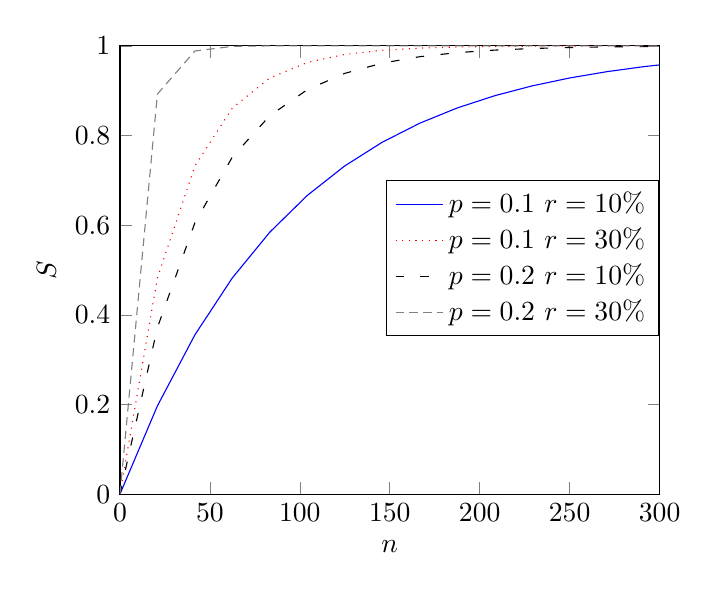
\begin{tikzpicture}
\begin{axis}[
    xlabel={$n$},
	ylabel={$S$},
	yticklabel style={/pgf/number format/fixed,
	    /pgf/number format/precision=1},
	xticklabel style={/pgf/number format/fixed,
	    /pgf/number format/precision=0},
	xmin = 0,
	xmax = 300,
	ymin = 0,
	ymax = 1.0,
	legend entries= {
	  $p=0.1\ r=10\%$, 
	  $p=0.1\ r=30\%$, 
	  $p=0.2\ r=10\%$,
	  $p=0.2\ r=30\%$,
	},
	legend style={at={(1,0.7)},anchor=north east}
]
\addplot[blue,solid,domain=0:500] { 1-exp(x*0.1*ln(1-0.1)) };
\addplot[red,dotted,domain=0:500] {1-exp(x*0.3*ln(1-0.1))};
\addplot[black,loosely dashed,domain=0:500] {1- exp(x*0.1*ln(1-0.2)) };
\addplot[gray,densely dashed,domain=0:500] { 1-exp(x*0.3*ln(1-0.3)) };
\end{axis}
\end{tikzpicture}
}
\bicaption[fig:ratePoss]{图索引}{一些情况下的正确性保证和有效搜索次数的关系}{Fig}{The relation between the assurance and query times}
\end{figure}

我们在图\ref{fig:ratePoss}中绘制了在几种特定云服务商欺骗率p和采样率r的情况下,用户能成功发现云服务商有问题的概率S和用户进行的有效搜素次数n的关系。这里,$S = 1 - (1-p)^{n \times p}$。从图中我们可以看出,随着搜索次数的增多,用户能发现云服务有问题的概率呈指数级增长。在云服务商欺骗率固定的情况下,采样率越高,正确性保证越高。在系统的实际使用中,我们可以考虑动态地调整采样率,比如说刚开始的时候使用较高的采样率,以期望能在更早的时候发现云服务是不是有问题,之后的使用中,可以降低采样率来取得更好的性能。同时,我们可以考虑将一些采样验证放在系统空闲时间进行,比如说放在深夜。

\section {大数据集的性能测试}
\begin{table}[htb]
    \centering
	\bicaption[tab:wiki_speedup]{表}{Wikipedia数据集上的性能测试结果}{Tab.}{The performance on dataset wikipedia}
    \begin{tabular}{cccccc}
        \toprule
        查询编号 & 耗时(s) \\
        \midrule
        1 & 706.038  \\
        2 & 8.096  \\
        3 & 209.649  \\
        4 & 7.677  \\
        5 & 770.438  \\
        6 & 87.117  \\
        \midrule
        平均 & 298.169  \\
        \bottomrule
    \end{tabular}
\end{table}
本测试我们使用的是Wikipedia数据集,在10台机器上进行。
各台机器上的模块部署情况如下:
\begin{itemize}
\item 机器0:Search Client、Search Server
\item 机器1:Correctness Server
\item 机器2:Integrity Server
\item 机器3 - 9:Query Node
\end{itemize}

测试结果如表格\ref{tab:wiki_speedup} 所示。从测试结果中,
我们可以看出我们的系统能够对100GB数据规模的数据集进行处理,
但处理速度还不是很好,而且不同查询的处理速度有着很大的变化。
对于有些查询,我们的系统能够在10秒内给出结果,而对于一些别的查询,
处理时间却长达10分钟。这主要的原因是,这些查询关键词的文档集合都是在百万千万级别的,且不同的关键词之间的文档集合差异很大。
对于这么大的集合,我们系统计算结果证明的速度还有待提高。

\section{本章小结}
在本章我们对云搜索正确性快速验证系统进行了一系列的实验评估。我们的实验使用了两个比较有代表性的数据集:Enron Email和Wikipedia。对系统的实验评估主要通过比较我们的系统和直接计算之间的性能差异进行。

首先,我们比较了使用树状结构证明前后正确性证明生成时间上的差异,实验结果表明使用树状结构证明对正确性证明生成速度有大约2.5倍的提升。接着,我们测试了系统的整体性能表现。实验结果表明我们的系统比直接计算的方法有着差不多2倍的性能提升。然后,我们比较了使用树状结构证明前后的验证时间差异。实验结果表明,使用了树状结构证明之后,验证时间有10\%左右的增加,处在可以接受的程度范围内。接着,我们对基于采样的验证机制进行了性能测试。实验结果表明使用了采样验证之后,系统的性能有着较大的提高。比如在10\%采样率时,系统的性能有着8倍左右的提高,而此时的系统正确性保证也是不错的。最后,我们在大数据集上进行了性能测试,测试结果表明我们的系统能够在大数据集上正常使用,但系统的效率还不够高。

\chapter{全文总结}
\label{chap:conclusion}

本文章介绍了一个云搜索的快速验证系统的原理和设计。为了解决目前云搜索没有什么合适的验证系统的问题,我们先是研究了一些目前的验证机制,选择了一个机遇RSA Accumulator的验证机制作为我们系统的基础。然后我们根据这个验证机制的特点,设计了一个高效的,具有不错扩展性的系统,并且对这个验证机制做了一些调优,比如设计了树状证明来进一步提高这个系统的效率。最后,我们使用了两个比较有代表性的数据集对我们的系统进行了实验测试。实验结果表明,我们的系统相比于原来验证机制的直接计算平均有两倍的速度提升,而且处理的数据规模变得更大了。总体来看,我们的系统可以用于一般的日常使用,但对于大数据集,我们系统的效率还有待提高。

在之后,我们可以尝试加快完整性证明的生成速度,比如说想办法做类似树状证明的任务拆解,是的完整性证明也可以并行的计算。我们也可以尝试使用GPU来加快证明生成过程的数学计算。希望能在今后实现一个更加高效,能处理更大规模数据的系统。

 %% 全文总结


%%%%%%%%%%%%%%%%%%%%%%%%%%%%%% 
%% 附录(章节编号重新计算,使用字母进行编号)
%%%%%%%%%%%%%%%%%%%%%%%%%%%%%% 
\appendix

% 附录中编号形式是"A-1"的样子
\renewcommand\theequation{\Alph{chapter}--\arabic{equation}}
\renewcommand\thefigure{\Alph{chapter}--\arabic{figure}}
\renewcommand\thetable{\Alph{chapter}--\arabic{table}}

%\include{body/app1} % 更新记录
%\include{body/app2} % 麦克斯韦方程
% \include{body/app3}


%%%%%%%%%%%%%%%%%%%%%%%%%%%%%% 
%% 文后(无章节编号)
%%%%%%%%%%%%%%%%%%%%%%%%%%%%%% 
\backmatter

% 参考文献
% 使用 BibTeX
% 包含参考文献文件.bib
\bibliography{ref}

%% 个人简历(硕士学位论文没有个人简历要求)
% \include{body/resume}

% 致谢
%%==================================================
%% thanks.tex for SJTU Master Thesis
%% based on CASthesis
%% modified by wei.jianwen@gmail.com
%% version: 0.3a
%% Encoding: UTF-8
%% last update: Dec 5th, 2010
%%==================================================

\begin{thanks}
光阴似箭,两年半的研究生生涯马上就要结束,同时也意味着我这十多年的求学生涯的结束,另一段人生篇章的开启。在读研的两年半时间里,有过欢笑也有过苦涩,经历过许许多多的挫折,也取得过多多少少的成绩。这一路走来,有很多感谢的话在心里,就让我趁着这个机会,说说心里感谢的话。

我要感谢我的导师赵建军老师和周憬宇老师。如果没有你们一直以来的谆谆教诲,也就不会有我现在的成绩。在学习和科研上,你们给了我非常珍贵的指导意见。在我遇到困难时,因为有你们的帮助,我从未孤立无援过。除了学业上的指导,你们更是教会了我要做一个什么样的人。你们在学术上严谨端正,对学生慈爱包容,对事业有着崇高的追求。这些都是我人生道路上最好的榜样。

我要感谢唐飞龙老师以及同在一个实验室的伙伴们。在5401实验室的这些日子里,承蒙有唐老师的照顾,我们才得有舒适的学习科研环境。在5401这个大家庭,我感受到了家一样的温暖,使得我可以心无旁骛地在学业的道路不断前行。

我要感谢我的朋友们。求学之路艰难,幸得你们相伴。希望不管时间走得多远,我们都永远不要走散。

我要感谢我的父母家人。我是一个不喜欢表达感情的人,所以也从来没和你们说过一声谢谢。但你们对我的无私关怀,我一直都记在心里。在以后的日子里,我会和你们一起承担家庭的责任,一起去面对人生的风风雨雨。

\end{thanks}


% 发表文章目录
%%==================================================
%% pub.tex for SJTU Master Thesis
%% based on CASthesis
%% modified by wei.jianwen@gmail.com
%% version: 0.3a
%% Encoding: UTF-8
%% last update: Dec 5th, 2010
%%==================================================

\begin{publications}{99}

    \item\textsc{Genguo W}. {A Fast Proof Generating System for Verifying Cloud Search}.
      International Conference on Information Technology and Electronic Commerce, 2014.

\end{publications}


% 参与项目列表
%\include{body/projects}

\end{document}
